\documentclass[14pt, fleqn, xcolor={dvipsnames, table}]{beamer}
\usepackage[T2A]{fontenc}
\usepackage[utf8]{inputenc}
\usepackage[english,russian]{babel}
\usepackage{amssymb,amsfonts,amsmath,mathtext}
\usepackage{cite,enumerate,float,indentfirst}
\usepackage{cancel}

\usepackage{tikz}                   
\usetikzlibrary{shadows}

% \usepackage{enumitem}
% \setitemize{label=\usebeamerfont*{itemize item}%
%   \usebeamercolor[fg]{itemize item}
%   \usebeamertemplate{itemize item}}

\graphicspath{{images/}}

\usetheme{Madrid}
\usecolortheme{seahorse}
\renewcommand{\CancelColor}{\color{red}}

\setbeamercolor{footline}{fg=Blue!50}
\setbeamertemplate{footline}{
  \leavevmode%
  \hbox{%
  \begin{beamercolorbox}[wd=.333333\paperwidth,ht=2.25ex,dp=1ex,center]{}%
    И. Кураленок, Н. Поваров, Яндекс
  \end{beamercolorbox}%
  \begin{beamercolorbox}[wd=.333333\paperwidth,ht=2.25ex,dp=1ex,center]{}%
    Санкт-Петербург, 2013
  \end{beamercolorbox}%
  \begin{beamercolorbox}[wd=.333333\paperwidth,ht=2.25ex,dp=1ex,right]{}%
  Стр. \insertframenumber{} из \inserttotalframenumber \hspace*{2ex}
  \end{beamercolorbox}}%
  \vskip0pt%
}
\newcommand\indentdisplays[1]{%
     \everydisplay{\addtolength\displayindent{#1}%
     \addtolength\displaywidth{-#1}}}
\newcommand{\itemi}{\item[\checkmark]}

\title{Машинное обучение: оценка методов обучения с учителем\\\small{}}
\author[]{\small{%
И.~Куралёнок,
Н.~Поваров}}
\date{}

\begin{document}

\begin{frame}
\maketitle
\small
\begin{center}
\vspace{-60pt}
\normalsize {\color{red}Я}ндекс \\
\vspace{80pt}
\footnotesize СПб, 2013
\end{center}
\end{frame}

\section{Постановка задачи и классификация способов оценки}
\begin{frame}{Задача на сегодня}
\emph{Задача:} Есть метод обучения и данные, на которых обучаемся. Хотим понять хорошо ли будет работать решающая функция на практике.\\

\flushleft{\em ``If you can't measure it, you can't improve it''} \\
\flushright{\textbf{—-- Lord Kelvin}} \\

\flushleft{\em ``Гораздо легче что-то измерить, чем понять, что именно вы измеряете.''} \\
\flushright{\textbf{—-- Джон Уильям Салливан}}
\end{frame}

\subsection{Источники проблемы}
\begin{frame}{Источник проблемы}
$$
F_0 = \arg \max_{F(D)} \mu_{\xi \sim U\left(\Gamma\right)}T(y_{\xi}, F(x_{\xi}))
$$
Мы обучаемся на одном множестве, а работаем на другом. А что, если эти множества отличаются?
\end{frame}

\begin{frame}{Свойства выборки}
\flushleft{\em ``Иными словами, репрезентативная выборка представляет собой микрокосм, меньшую по размеру, но точную модель генеральной совокупности, которую она должна отражать.''}\\
\flushright{\textbf{--- Дж. Б. Мангейм, Р. К. Рич}}\\
\flushleft
Такого сложно достичь, поэтому хотим лишь ``несмещенности'' по параметрам обучения:
\small
$$\begin{array}{rl}
F_0 =& \arg \max_{F} \mu_{\xi \sim U(D)} T(y_{\xi}, F(x_{\xi})) \\
    =& \arg \max_{F} \mu_{\xi \sim U(\Gamma)} T(y_{\xi}, F(x_{\xi}))
\end{array}$$
\end{frame}


\subsection{Классификация способов оценки}
\begin{frame}{Способы повлиять на несмещенность}
Интересно получить выборку, несмещенную (смещенную не более чем $\ldots$) по результатам процедуры обучения:
\begin{itemize}
 \item Найти «хороший» способ генерации выборки при условии процедуры подбора
 \item Наложить ограничения на процедуру подбора
 \item Ограничения на решающую функцию
\end{itemize}
$\Rightarrow$ \textbf{Надо научиться мерять смещенность выборки, и чем тоньше изменения, тем более точный инструмент измерения нужен.}
\end{frame}

\begin{frame}{Известные способы оценки}
Оценка по принципу ``чёрного ящика'':
\begin{itemize}
  \item Оценка в боевых условиях (на пользователях)
  \item Кросс-валидация
  \item Повторные выборки
\end{itemize}
Оценка по принципу ``прозрачного ящика'':
\begin{itemize}
  \item VС-оценки
  \item PAC-Bayes bounds
  \item Оценки по Воронцову
\end{itemize}
\end{frame}

\section{Black box оценка}
\begin{frame}{Оценка в боевых условиях}
Как оценить, насколько пользователяю системы ``хорошо'' по его поведению?
Конкретная реализация зависит от области, но можно выделить типы:
\begin{itemize}
\item blind testing;
\item A/B тестирование (Abandonment Rate, MRR by long clicks, etc.);
\item подстроенные результаты (TDI, BI, etc.).
\end{itemize}
\footnotesize Мы можем долго-долго рассказывать байки в этом месте :).
\end{frame}

\subsection{Cross-validation}

\begin{frame}{Cross-fold validation I}
Разобьем множество $X$ на два $L$ и $T$ так, чтобы $L \cup T = X, L \cap T = \emptyset$ случайным образом (Jackknife).
Будем обучаться на одной половине а проверять результат обучения на другой.
\begin{description}
\itemindent=0em
\labelwidth=0em
\leftskip=-3em
  \item[\color{green}+] простой и надежный
  \item[\color{green}+] позволяет оценить распределение на множестве решений
  \item[\color{red}--] последовательные эксперименты зависимы
  \item[\color{red}--] используем мало данных для обучения
  \item[\color{red}--] непонятно как подбирать соотношения $\frac{|L|}{|T|}$
\end{description}
\end{frame}

\begin{frame}{Cross-fold validation II}
Можно организовать разными способами:
\begin{description}
\itemindent=0em
\labelwidth=0em
\leftskip=-3em
  \item[2-fold] обычно так и делаем
  \item[k-fold] когда очень боимся зависимости экспериментов, а данных много
  \item[Leave-one-out (LOO)] когда совсем мало данных
\end{description}
\end{frame}


\begin{frame}{Повторные выборки}
В статисике продолжением метода Jackknife стал Bootstrapping.
Сформируем 2 множества $L$ и $T$ так, что:
\begin{enumerate}
  \item $|L| = |T| = |X|$
  \item $l_i \sim U(X), t_i \sim U(X)$
\end{enumerate}
Будем считать, что эти 2 множества разные.
\begin{description}
\itemindent=0em
\labelwidth=0em
\leftskip=-3em
  \item[\color{green}+] используем полный объем выборки
  \item[\color{green}+] на больших объемах вариативность выбора огромна
  \item[\color{red}--] теперь еще и $T$ зависит от $L$ и как это учесть -- не ясно
\end{description}
$\Rightarrow$ можно применять только на больших объемах (>10k точек)
\end{frame}

\begin{frame}{Как принять решение по результатам CV/ПВ}
Не стоит забывать, что результаты CV/ПВ экспериментов всегда {\color{red} \em зависимы}, и не спасают нас от смещенности исходной выборки.
\small
\begin{enumerate}
  \item провести серию последовательных эксприментов;
  \item закрыв глаза на зависимость, построить доверительные интервалы на $T(F_0, T)$;
  \item чтобы сравнить два альтернативных метода можно проверить
  $$H_0: \mu\left(T(F_{0_A}, T)\right) = \mu\left(T(F_{0_B}, T)\right)$$
  например с помощью парного WX-test'а.
\end{enumerate}

\end{frame}

\section{Сложность модели}
\subsection{Пример с полиномами}

\begin{frame}{Сложность модели}{}
{\em Чем больше в модели параметров, тем большую информацию они несут.}\\
\flushright{\bf --- Ваш К.О.}
\flushleft\small
Какая бывает информация в параметрах:
\begin{itemize}
  \item про генеральную совокупность;
  \item про выборку;
  \item про random seed.
\end{itemize}
Если мы будем усложнять модель, соотношения информации будут двигаться.\\

\textbf{$\Rightarrow$ Хотим придумать рычажок, который контролирует сложность модели.}
\end{frame}

\begin{frame}{Семейство полиномов $p$-й степени}
Будем строить семейства решающих функций следующим образом:
\small
$$\begin{array}{l}
F(x, \lambda_1=\{w\}) = w^Tx \\
F(x, \lambda_2=\{w,A\}) = w^Tx + x^TAx\\
F(x, \lambda_3=\{w,A,B\}) = w^Tx + x^TAx + \sum_i\sum_j\sum_k b_{ijk} x_i x_j x_k\\
etc.\\
\end{array}$$
Понятно, что $|\lambda_i| < |\lambda_{i+1}|$.
\end{frame}

\subsection{VC-dimension}
\begin{frame}{Размерность Вапника-Червоненкиса}
\begin{definition}[ru.wikipedia.org]
$VC$-размерность класса функций $F$ --- наибольшее количество точек, которое может быть разделено функциями семейства, вне зависимости от конфигурации множества точек.
\end{definition}
\begin{tabular}{p{0.70\textwidth}p{0.25\textwidth}}
\colorbox{green!10}{
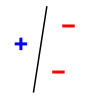
\includegraphics[width=0.20\textwidth]{100px-VC1.png}\hspace{2px}
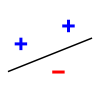
\includegraphics[width=0.20\textwidth]{100px-VC2.png}\hspace{2px}
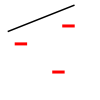
\includegraphics[width=0.20\textwidth]{100px-VC3.png}\hspace{1px}
} & \colorbox{red!10}{
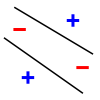
\includegraphics[width=0.20\textwidth]{100px-VC4.png}\hspace{1px}
} \\
\end{tabular}
{\footnotesize картинки с en.wikipedia.org}
\end{frame}

\section{Виды ошибок}
\begin{frame}{Overfit vs. underfit}
\centering
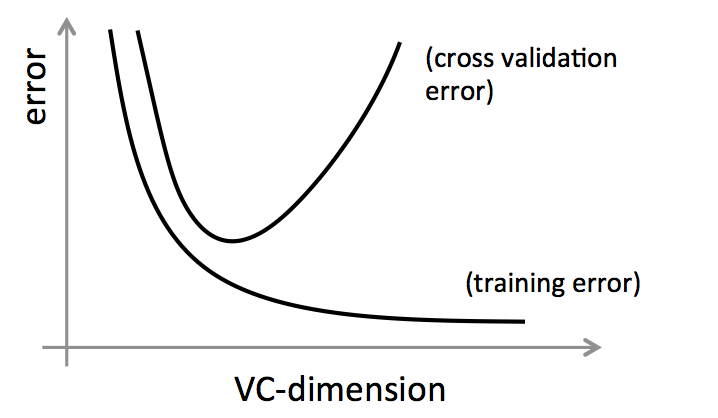
\includegraphics[width=0.8\textwidth]{overfit_underfit.png} 
\end{frame}

\begin{frame}{Overfit vs. underfit определения}
\small
\begin{description}
\leftmargin=-5em
\itemindent=0em
\labelwidth=0em
\leftskip=-5em
  \item[Переобучение, переподгонка (overtraining, overfitting)] —-- нежелательное явление, возникающее при решении задач обучения по прецедентам, когда вероятность ошибки обученного алгоритма на объектах тестовой выборки оказывается существенно выше, чем средняя ошибка на обучающей выборке. 
  \item[Недообучение (underfitting)] --- нежелательное явление, возникающее при решении задач обучения по прецедентам, когда алгоритм обучения не обеспечивает достаточно малой величины средней ошибки на обучающей выборке. Недообучение возникает при использовании недостаточно сложных моделей.
\end{description}
\flushright{\bf \normalsize--- machinelearning.ru}
\end{frame}

\begin{frame}{Как это выглядит в полиномах (underfit)}
\begin{center}
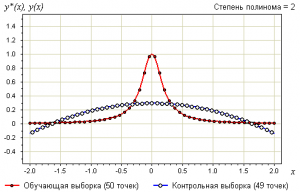
\includegraphics[width=0.9\textwidth]{300px-LsmRunge2.png}
\end{center}
{\footnotesize картинка с machinelearning.ru}
\end{frame}

\begin{frame}{Как это выглядит в полиномах (fit)}
\begin{center}
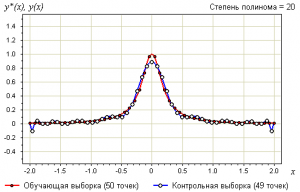
\includegraphics[width=0.9\textwidth]{300px-LsmRunge20.png}
\end{center}
{\footnotesize картинка с machinelearning.ru}
\end{frame}

\begin{frame}{Как это выглядит в полиномах (overfit)}
\begin{center}
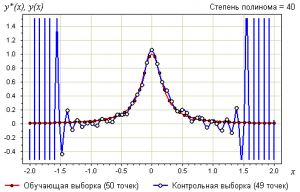
\includegraphics[width=0.9\textwidth]{300px-LsmRunge40.png}
\end{center}
{\footnotesize картинка с machinelearning.ru}
\end{frame}

\begin{frame}{Как это выглядит в пространстве решений}
\centering
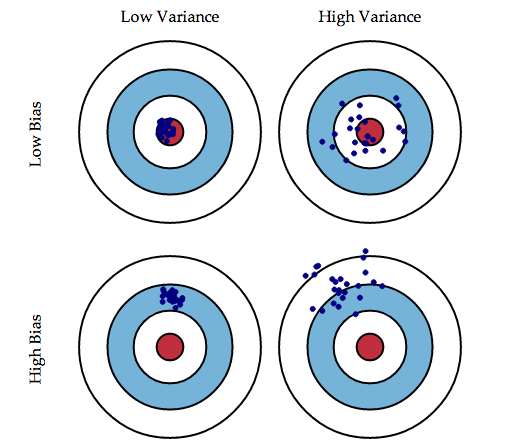
\includegraphics[width=0.65\textwidth]{bias_variance.png} 
\end{frame}

\begin{frame}{Что в какой ситуации делать}
\begin{itemize}
  \item Увеличение числа примеров для обучения фиксят high variance, но не high bias
  \item Меньшее число факторов фиксят high variance, но не high bias
  \item Увеличение числа факторов фиксят high bias, но не high variance
  \item Добавление степени к полиному и взаимодействующих факторов фиксят high bias, но не high variance
\end{itemize}
\end{frame}

\begin{frame}{Понимаем в какой ситуации находимся}
\centering
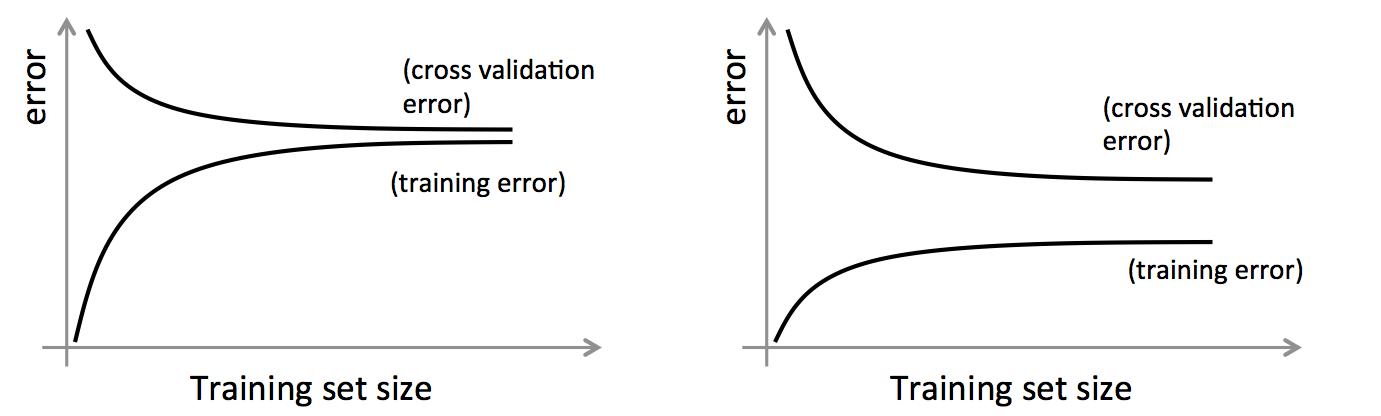
\includegraphics[width=1.0\textwidth]{bias_error.png}
\end{frame}

\begin{frame}{Понимаем в какой ситуации находимся}
\centering
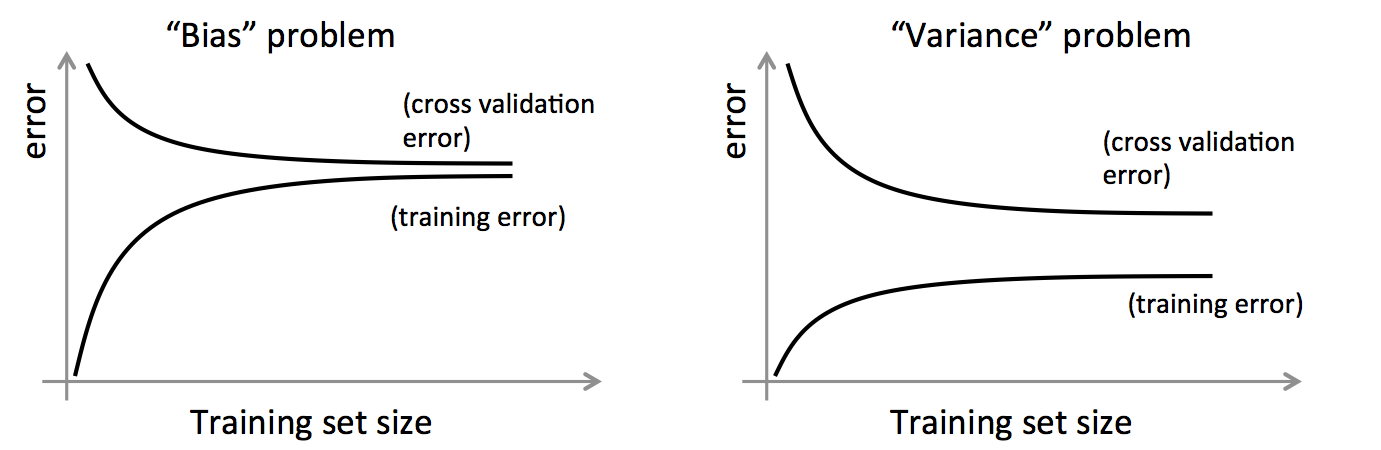
\includegraphics[width=1.0\textwidth]{bias_error_2.png}
\end{frame}


\section{Glass box оценка}
\begin{frame}{Теоретическая оценка}
Цели оценки:
\begin{itemize}
  \item Можно ли понять какой метод круче для заданного объема данных
  \item Предсказать сложность на которой достигается fit
\end{itemize}
Будем рассматривать задачу классификации и определять долю ошибок ($T = -\sum_i I(y_i \ne F(x_i))$). 
\end{frame}

\subsection{VC-оценка и ее применение}
\begin{frame}{Русские тоже что-то могут в ML :)}
Владимир Наумович Вапник (NEC\footnote{Здесь и далее по данным ru.wikipedia.org}), \\
Алексей Яковлевич Червоненкис (University of London). \\
Разработали первую теорию по оценке переобучения в зависимости от класса решающих функций в 60-70е годы.
\end{frame}

\begin{frame}{Оценка по методу Вапника-Червоненкиса I}
Хотим оценить $T(T)$ сверху по $T(L)$ и свойствам семейства решающих функций.\\
$$
T(T) \ge T(L) - \sqrt{h(\log(\frac{2n}{h})+1)-\log(\frac{\eta}{4})\over n}
$$
с вероятностью $1-\eta$, где $h$ -- $VC$-оценка семейства, $n = |L|$.
\end{frame}

\begin{frame}{Оценка по методу Вапника-Червоненкиса II}
\begin{center}
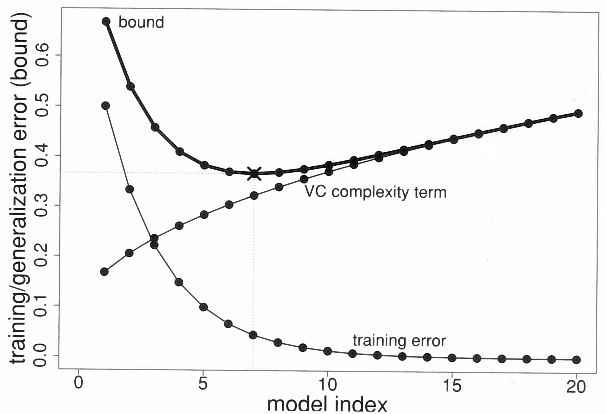
\includegraphics[height=0.6\textheight]{Herbrich2002_4-4.png}
\end{center}
{\footnotesize картинка с www.svms.org}
\end{frame}

\subsection{PAC-Bayes bounds I}
\begin{frame}{PAC-Bayes bounds I}
\small
Кажется, что не все определяет только $VC$-размерность. Для одних данных работают одни решения, для других -- другие. \\
\begin{definition}[Оценка McAllester'а (1998)]
Введем априорное распределение над семейством решающих функций $F$. Тогда:
$$
T(F_0, T) \ge T(F_0, L) - \sqrt{log \frac{1}{p(F_0)} + log(\frac{1}{\eta}) \over 2n}
$$
с вероятностью не меньше $1-\eta$.
\end{definition}
\end{frame}

\begin{frame}{PAC-Bayes bounds II}
\small
Рассмотрим решение, как взвешивание между разными функциями семейства $F$.\footnote{Это такое байесовское решение, о котором мы поговорим в следующий раз} Тогда получится еще краше (современный вид):
$$
|\mu_\rho T(F_i, T) - \mu_\rho T(F_i, L)| \ge \sqrt{KL(\rho \| \pi) + log \frac{4n}{\eta} \over 2n - 1}
$$
с вероятностью не меньше $1-\eta$, где $\rho$ --- априорное распределение в семействе $F$, $\pi$ --- апостериорное.
\end{frame}

\subsection{Оценка в слабой аксиоматике Воронцова}
\begin{frame}{Оценка в слабой аксиоматике Воронцова}
Воронцов Константин Вячеславович (ШАД в Москве, machinelearning.ru) написал докторскую диссертацию на тему \\
\center{\textit{``Комбинаторная теория надёжности обучения по прецедентам''}} \\
\flushleft в которой предложил интересную альтернативу VC-оценкам и PAC-Bayes.
\end{frame}

\section{Про неточные решения}
\begin{frame}{Соображения об точности решения}
До этого мы говорили о точных решениях. Но точность определения параметров обучения определяет количество информации в решении. \\
$\Rightarrow$ Не надо вычислять параметры решения до 100-го знака: sizeof(long double) >> sizeof(float) \\
~\\
В задачах итеративной оптимизации мы привыкли устремлять шаг к 0, что в случае ML приводит к большему variance решений.
\end{frame}

\section{Overfit on validate}
\begin{frame}{Как еще можно переобучиться?}
Будем долго и упорно подбирать метод обучения на фиксированном делении $L, T$:
$$
\max_{i} \left(\arg\max_{f \in F_i} T(f, L)\right)(T)
$$
Это же максимизация на всем множестве $L \cup T = X$! Называется такое overfit on validate. Что с этим делать? Исследовать
$$
\cancel{\max} \left(\arg \max_{i} \left(\arg\max_{f \in F_i} T(f, L)\right)(V)\right)(T)
$$
\end{frame}

\section{Где брать данные}
\begin{frame}{Где взять данные для экспериментов}
\begin{itemize}
  \item Реальные данные
  \begin{itemize}
    \item Поиск: РОМИП, TREC, Яндекс.ИМАТ, Yahoo LTRCh
    \item Pascal Challenge
    \item InnoCentive
    \item Kaggle
  \end{itemize}
  \item Синтетические данные (многомерный XOR)
  \item ``Загадки'': задумаем «хитрое» распределение и попробуем его отгадать
\end{itemize}
\end{frame}

\section{Домашнее задание}
\begin{frame}{Задача}
Дано:
\begin{itemize}
  \item $L$ = 1000 точек, полученных по правилу:
$$\begin{array}{l}
x \sim U (0,10] \\
y = ln(x)
\end{array}$$
  \item $T$ = 10000 реализаций $x$ для которых надо найти~$y$
\end{itemize}
Задача: найти решение в классе полиномов оптимальной степени $p$, наилучшим образом приближающий $y$ на $T$.

\end{frame}

\begin{frame}{Где брать домашние задания}
\begin{itemize}
  \item svn checkout http://ml-lections.googlecode.com/svn/trunk/ ml-lections-read-only
  \item Комитить не получится ;)
  \item Бонусом - лекции в tex.
  \item Лекции находятся в разных папках. В папке лекции есть папка homework.
  \item Помимо датасетов содержат файл howto.txt
  \item Вопросы: saintnik@yandex-team.ru
\end{itemize}

\end{frame}

\end{document} 
